\documentclass[a4paper]{article}
\usepackage{times}
\usepackage[utf8]{inputenc}
\usepackage[T1]{fontenc}
\usepackage{graphicx}
\usepackage{amssymb}
\usepackage{hyperref}
\linespread{1.5}	% double spaces lines
\usepackage[hmargin=3cm,vmargin=3cm]{geometry}
\usepackage{indentfirst}
\usepackage{amsmath}
\usepackage{amsthm}
\usepackage{sectsty}
\usepackage{enumitem}
\usepackage[brazil]{babel}
\usepackage{placeins} %mantem figuras na secao com \FloatBarrier
\usepackage{fixltx2e} %\textsubscript
\usepackage{textcomp}
\hypersetup{%
    pdfborder = {0 0 0}
}

\begin{document}

\begin{titlepage}
\begin{center}


\large{ 
\uppercase{ Universidade Federal do Rio Grande do Sul\\

Instituto de Informática \\

Curso de Ciência da Computação \\

Circuitos Digitais (2014/1)\\
}

Prof. Dr. Marcelo de Oliveira Johann \\

Graduandos: \\ Paulo Renato Lanzarin (228818)
			\\ Ricardo Gabriel Herdt (160622) \\ [4.5cm]


% Title
\LARGE {\bfseries Relatório do laboratório 07: \\
	Projeto de multiplexador e decodificador\\[1.0cm]
}}


\vfill

Porto Alegre, 01 de Maiol de 2014

\end{center}
\end{titlepage}
\section{Descrição}

	O projeto deste laboratório consistiu na elaboração de um decodificador de 4 para 16 e um multiplexador de 8 para 16, ambos desenvolvidos na ferramenta \emph{Max+plus II}. O decodificador, de entradas a[3..0], realiza a decodificação através de 16 portas OR que selecionam  as combinações binárias das entradas (0000, 0001, ..., 1111) em saídas b[15..0]. O multiplexador, por sua vez, foi desenvolvido em partes: primeiramente, foi projetado um MUX 2:1 com um sinal de seleção, entradas d[1..0] e saída a0 utilizando duas portas AND e uma OR selecionando as entradas. Tal MUX foi definido como um bloco e utilizado para compor o multiplexador 8:16, que nada mais é que oito MUX2:1 dispostos com um mesmo sinal de seleção s0.



\FloatBarrier

\section{Circuitos}

	Os diagramas esquemáticos dos circuitos projetados neste laboratorio estão como seguem nas subseções.

\subsection{Decodificador de 4 para 16}

	Como dito na descrição do experimento, o decodificador é como o exposto no diagrama esquemático a seguir:
\begin{figure}[h!]
  \centering
  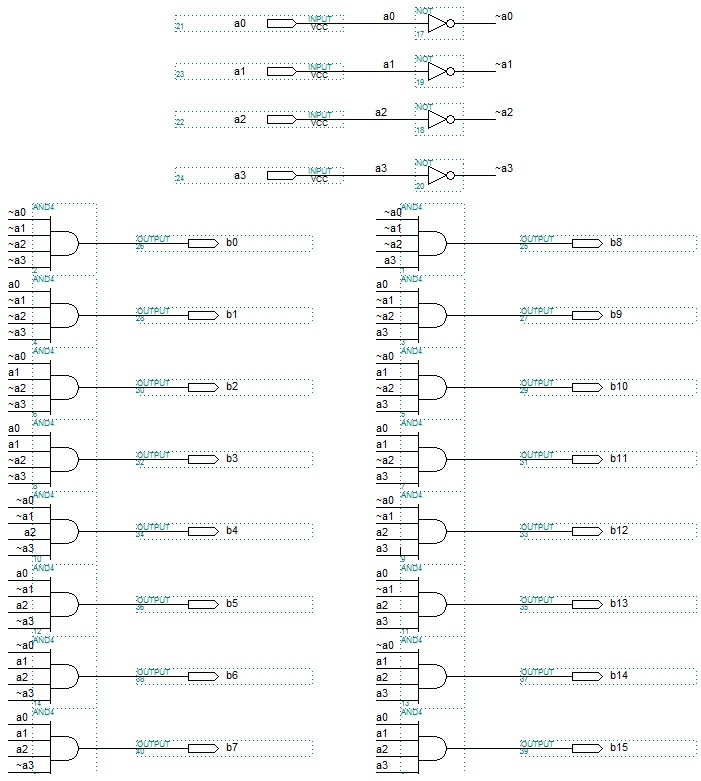
\includegraphics[scale=0.53]{decod_4-16(2).jpg}
  \caption{Diagrama esquemático do DEC4:16 retirado do \emph{Max+plus II}}
\end{figure}



\FloatBarrier

\subsection{Mutiplexador de 8 para 16}
	O MUX2:1 utilizado na composição do MUX8:16 é tal qual esta no diagrama a seguir:
\begin{figure}[h]
  \centering
  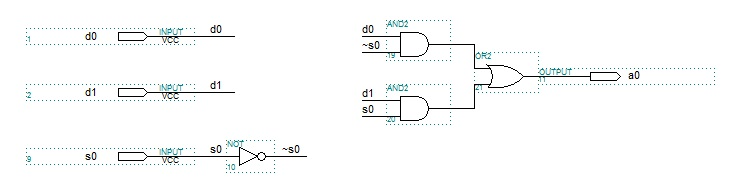
\includegraphics[scale=0.9]{mux_2-1.jpg}
  \caption{Diagrama esquemático do MUX2:1 retirado do \emph{Max+plus II}}
\end{figure}



\FloatBarrier

\section{Simulação}

A simulação funcional dos circuitos projetados estão expostas nas subseções seguintes e foram retiradas do \emph{Max+plus II}.

\subsection{Simulação do decodificador de 4 para 16}
\begin{figure}[h]
  \centering
  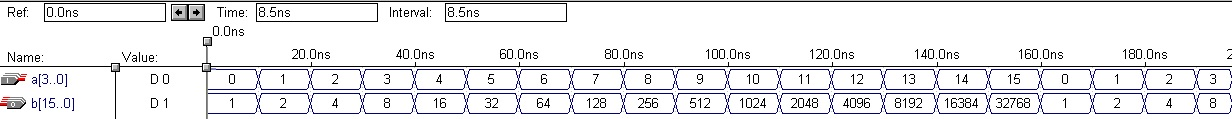
\includegraphics[scale=0.5]{lab07_simulacao_decodificador.jpg}
  \caption{Simulação funcional do DEC4:16}
\end{figure}



\FloatBarrier

\subsection{Simulação do multiplexador de 8 para 16}




\FloatBarrier



\FloatBarrier

\section{Conclusão}
O experimento foi importante ao concretizar a noção  de otimização de circuitos através da minimização por mapas de Karnaugh. Entrentanto, nota-se que isto foi possível levando em conta que o projeto em questao é de um circuito relativamente simples e, para algo mais complexo, seria impraticável proceder desta maneira.

\end{document}
